% EJB
\ifbook{
    \mysubsubsection{Propos de cette section}

    \paragraph{} Comme l'a expliciter, dans les premiers chapitres, la description des nombreux
    "conteneurs d'exécutions" dans lesquelles les applications modernes s'exécutent, il existe déjà
    un grand nombre de mécanismes que ces dernières peuvent utiliser, associés aussi à des certaines
    contraintes de programmation. Malgré, la réalisation d'application reste un sujet vaste, et il
    est fréquent que, dans le cadre d'un projet, on décide d'utilise un ou plusieurs autres
    \textit{framework} supplémentaire, fournissant généralement un cadre de développement estimé
    plus efficase pour l'implémentation désirée.

    \paragraph{} Rien que dans le monde Java, on distingue une kyrielle vertigineuse de ces
    \textit{frameworks} parmi lesquelles on citera juste les suivants:

    \begin{itemize}
      \item \mylink{TODO}{Spring}: un cavenas très développé conçu pour donner un cadre robuste et
      complet aux développement d'applications modernes. Il est souvent présenté comme une
      alternative simple à l'utilisation des standard associés à JEE.
      \item \mylink{TODO}{Struts}: un très célèbre \textit{framework} adaptant le classique modèle
      \mylink{TODO}{MVC} à la réalisation d'application \textit{web}.
      \item \mylink{TODO}{JSF} et ses implémentations: standard issu du monde JEE, JSF propose un
      un modèle de programmation dédié à la réalisation d'application \textit{web} métiers. Un des
      objectifs avoués du standard et de ses implémentations est de permettre un développement
      similaire à celui d'application dites "lourdes", en prenant en charge, autant que possible,
      les spécialités des technologies internet.
      \item ...
   \end{itemize}

   \paragraph{} Fort de ce simple constat, il apparait évident que dresser un tabelau exhaustif,
   même limiter à l'univers Java/JEE Open Source et standard, formerait une excellente treizième
   tâche pour Hercule, et dépasserait totaltement le cadre de cette exposé.

   \paragraph{} Néanmoins, ce genre de composant formant une partie intégrante du paysage associé
   aux \textit{middleware}, il est pertinent, dans le cadre de cours, de présenter l'un d'eux. Cette
   analyse donnera, espérons-le, au lecteur, une grille d'analyse suffisante pour entreprendre lui
   même ce travail de décorticage technologie lorsqu'il sera confronté à la toute dernière
   déclinaison "à la mode" de ces \textit{framework}.

   \paragraph{} Cette section présente donc, de manière volontairement très sommaire, les grandes
   lignes du modèle de programmation promût par le standard EJB, dans sa troisième version, de loin
   à ce jour la plus simple et réussi. L'objectif de ce standard, et de ses implémentations, est
   donc - comme nous allons le voir, la normalisation de la définition et utilisation de
   \textbf{composant distribué}.

   \paragraph{} \textit{Le lecteur prendra soin de noter immédiatement l'importance de bien saisir
   quel est l'objectif que cherche à atteindre le \textif{framework} et quel modèle de programmation
   il promeut. En effet, il est, de manière très regrettable et surtout dommageable, fréquent de
   voir des projets embarqués une kyrielle de composants, plus ou moins standard, plus ou moins
   ouvert, plus ou moins robustes, mais surtout plus ou moins utile à l'application. Cette
   empilement technologique confus, au delà de rendre le code de l'application très complexe, a
   aussi l'effort de bord d'augmenter grandement la difficulté de sa mise en oeuvre.}
}

\ifslide{

  \begin{frame}{Exemple de modèle de programmation: EJB}
    \begin{center}
      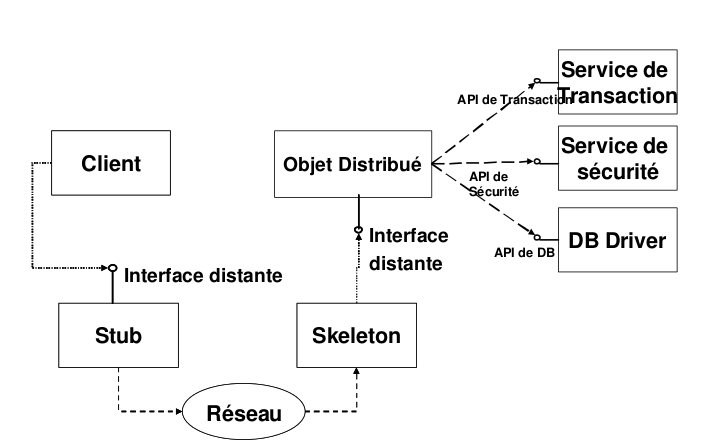
\includegraphics[scale=0.3]{img/ejb-overview.png}
    \end{center}
  \end{frame}
}



\begin{frame}
  \begin{block}{Motivations}
    \begin{itemize}
      \item EJB définit des contrats associés à un Bean
      \item Déploiement local ou distant
    \end{itemize}
  \end{block}

  \begin{block}{Standard}
     \begin{itemize}
       \item Portabilité des beans sur différents serveurs EJB
       \item Indépendance du fournisseur
    \end{itemize}
  \end{block}
\end{frame}

\begin{frame}
  \begin{block}{Types}
    \begin{itemize}
      \item Session Bean
      \item Entity Bean
      \item Message-Driven Bean
    \end{itemize}
  \end{block}

  \begin{center}
    Si l'on utilise un Session Bean quel impact sur l'architecture de l'application ?
  \end{center}

\end{frame}
